\section{Iterative center of mass displacement compensation algorithm}
In reality, the distribution of center of mass of the body is not known, and therefore, analytic solution give with (\ref{eq:CMsolution}) is impossible. Thus an iterative method, based on hopping response is proposed. When a quadruped is hopping, its contact with the ground is infitesimally short, and consequently, reaction forces and torques are approximated with the Dirac function $\delta (s)$. During the jump, the body behaves according to Euler body dynamics function (\ref{eq:EulerBody}). Taking account the infitessimally short time the body has to accelerate the cross coupling term $\vec{\omega}\times J_B\vec{\omega}$ can be neglected and the rotation speed vector can be approximated with (\ref{eq:RotSpeedAprox}).
\begin{figure}
	\centering
	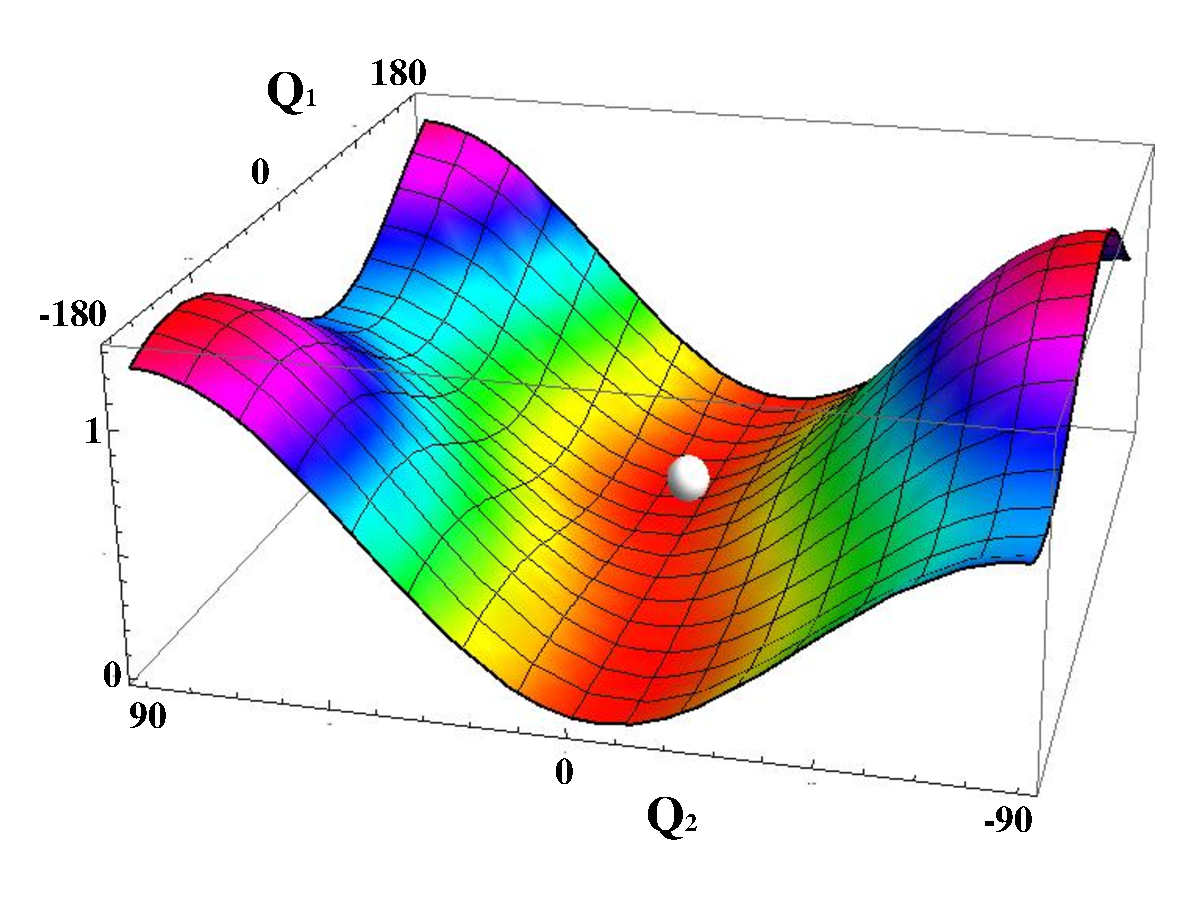
\includegraphics[width=85mm]{./pictures/RobinRepicCM.pdf}
	\caption{Center of mass displacement}
	\label{fig:rmoment}
\end{figure}

\begin{equation}\label{eq:EulerBody}
\tau_{tot}=J_B\vec{\dot{\omega}}+\vec{\omega}\times J_B\vec{\omega}
\end{equation}

\begin{equation}\label{eq:RotSpeedAprox}
\vec{\omega}\approx \frac{1}{s}{J_B}^{-1}\begin{bmatrix}
\Delta \textsc{cm}_y & -\Delta \textsc{cm}_x & 0
\end{bmatrix}^T\bar{T}\delta(s)
\end{equation}

Calculating the distance of vector (\ref{eq:RotSpeedAprox}) it is easy to show how the size of rotation speed vector is proportional to the displacement of center of mass. This effectively shows how moving the displacement of center of mass to the construction center of the robot eliminates the generation of unwanted rotations. 

\begin{equation}
\left \| \vec{\omega} \right \|\sim \sqrt{{\Delta \textsc{cm}_x}^2+{\Delta \textsc{cm}_y}^2}
\end{equation}


In order to iteratively calculate the angles $q1$ and $q2$, angular velocity vector is recorded during start of hopping acceleration phase $F_1$. This phase lasts until one of the leg/spring reaches desired length $L_d$. The leg which carries a minimum mass will achieve the fastest acceleration and the algorithm task is to navigate tail towards this leg. 

For example, mass distribution in figure  (\ref{fig:imassCom}) is equally distributed except for $MASS_2$  which is lighter then others. At the end of phase $F_1$ the body rotates at an angular velocity $\vec{\omega}$. By using the cross product of projection vector $\vec{\omega_{xy}}$ in $XY$ plane and body $\vec{Zb}$, the tail direction vector $\vec{\omega_{TD}}$ is calculated. 

Tail motion control algorithm navigates tail in vector $\vec{\omega_{TD}}$ direction which at the end results the equal mass distribution.

\begin{figure}
	\centering
	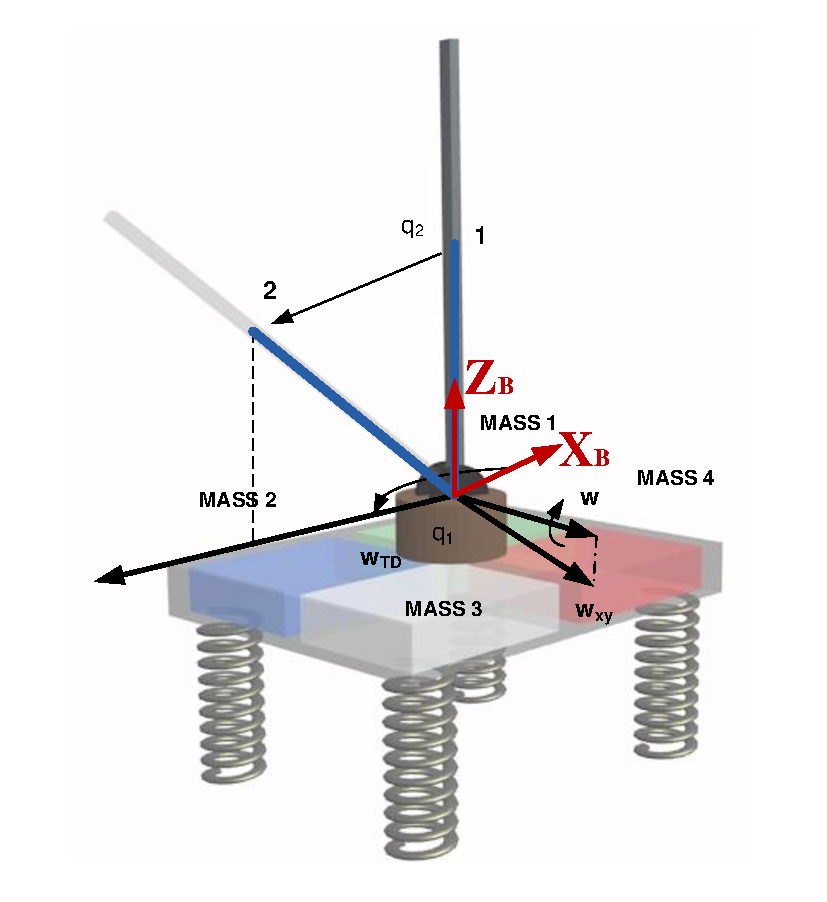
\includegraphics[width=85mm]{./pictures/IterativeAlgorithm.pdf}
	\caption{Iterative mass displacement compensation}
	\label{fig:imassCom}
\end{figure}





Due to the tail's infitesimal thickness, its moment of inertia, written in this frame can be simplified:
\begin{equation}
J_T=J_3=\frac{{Q_3}^2 m_3}{12}\left(
\begin{array}{ccc}
 1 & 0 & 0 \\
 0 & 1 & 0 \\
 0 & 0 & 0
\end{array}
\right)
\end{equation} 
\small
\begin{equation}
{J_T}^*={R_0^3}^TJ_TR_0^3+m_T\begin{bmatrix}
{cm_y^T}^2 +{cm_z^T}^2& {cm_x^T}{cm_y^T}& {cm_x^T}{cm_z^T} \\ 
-{cm_x^T}{cm_y^T} & {cm_x^T}^2+{cm_z^T}^2 & {cm_y^T}{cm_z^T}\\ 
-{cm_x^T}{cm_z^T} & -{cm_y^T}{cm_z^T} & {cm_x^T}^2+{cm_y^T}^2
\end{bmatrix}
\end{equation}
\normalsize
